\documentclass{extbook}[14pt]
\usepackage{multicol, enumerate, enumitem, hyperref, color, soul, setspace, parskip, fancyhdr, amssymb, amsthm, amsmath, bbm, latexsym, units, mathtools}
\everymath{\displaystyle}
\usepackage[headsep=0.5cm,headheight=0cm, left=1 in,right= 1 in,top= 1 in,bottom= 1 in]{geometry}
\usepackage{dashrule}  % Package to use the command below to create lines between items
\newcommand{\litem}[1]{\item #1

\rule{\textwidth}{0.4pt}}
\pagestyle{fancy}
\lhead{}
\chead{Answer Key for Module6 Version C}
\rhead{}
\lfoot{9356-6875}
\cfoot{}
\rfoot{testing}
\begin{document}
\textbf{This key should allow you to understand why you choose the option you did (beyond just getting a question right or wrong). \href{https://xronos.clas.ufl.edu/mac1105spring2020/courseDescriptionAndMisc/Exams/LearningFromResults}{More instructions on how to use this key can be found here}.}

\textbf{If you have a suggestion to make the keys better, \href{https://forms.gle/CZkbZmPbC9XALEE88}{please fill out the short survey here}.}

\textit{Note: This key is auto-generated and may contain issues and/or errors. The keys are reviewed after each exam to ensure grading is done accurately. If there are issues (like duplicate options), they are noted in the offline gradebook. The keys are a work-in-progress to give students as many resources to improve as possible.}

\rule{\textwidth}{0.4pt}

\begin{enumerate}\litem{
Describe the end behavior of the polynomial below.
\[ f(x) = -3(x - 8)^{5}(x + 8)^{10}(x - 6)^{3}(x + 6)^{5} \]The solution is the graph below, which is option A.
\begin{center}
    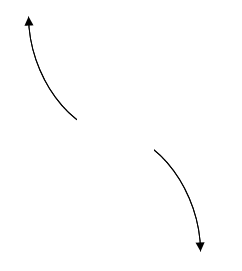
\includegraphics[width=0.3\textwidth]{../Figures/polyEndBehaviorAC.png}
\end{center}\begin{enumerate}[label=\Alph*.]
\begin{multicols}{2}
\item 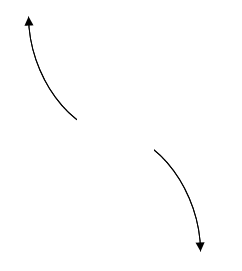
\includegraphics[width = 0.3\textwidth]{../Figures/polyEndBehaviorAC.png}
\item 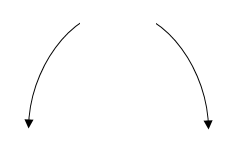
\includegraphics[width = 0.3\textwidth]{../Figures/polyEndBehaviorBC.png}
\item 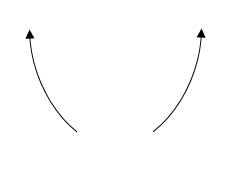
\includegraphics[width = 0.3\textwidth]{../Figures/polyEndBehaviorCC.png}
\item 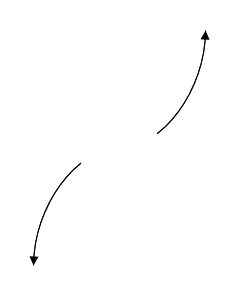
\includegraphics[width = 0.3\textwidth]{../Figures/polyEndBehaviorDC.png}
\end{multicols}\item None of the above.\end{enumerate}
\textbf{General Comment:} Remember that end behavior is determined by the leading coefficient AND whether the \textbf{sum} of the multiplicities is positive or negative.
}
\litem{
Which of the following equations \textit{could} be of the graph presented below?

\begin{center}
    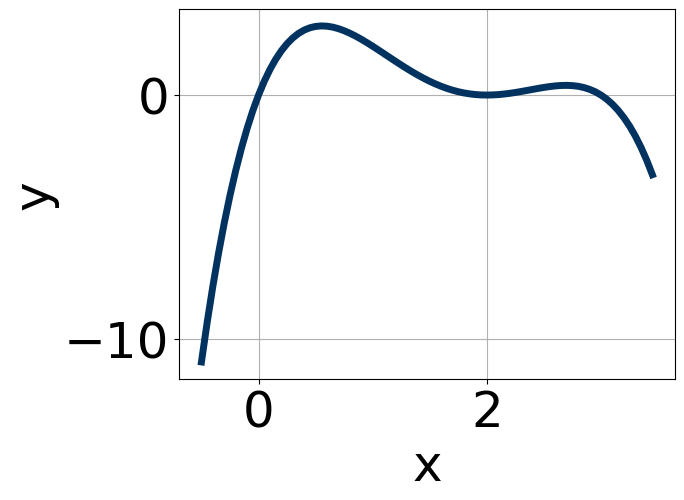
\includegraphics[width=0.5\textwidth]{../Figures/polyGraphToFunctionC.png}
\end{center}


The solution is \( -13x^{5} (x - 2)^{8} (x - 3)^{9} \), which is option E.\begin{enumerate}[label=\Alph*.]
\item \( 20x^{9} (x - 2)^{6} (x - 3)^{6} \)

The factor $(x - 3)$ should have an odd power and the leading coefficient should be the opposite sign.
\item \( -3x^{6} (x - 2)^{11} (x - 3)^{11} \)

The factor $2$ should have an even power and the factor $0$ should have an odd power.
\item \( 14x^{9} (x - 2)^{6} (x - 3)^{7} \)

This corresponds to the leading coefficient being the opposite value than it should be.
\item \( -19x^{6} (x - 2)^{10} (x - 3)^{9} \)

The factor $x$ should have an odd power.
\item \( -13x^{5} (x - 2)^{8} (x - 3)^{9} \)

* This is the correct option.
\end{enumerate}

\textbf{General Comment:} General Comments: Draw the x-axis to determine which zeros are touching (and so have even multiplicity) or cross (and have odd multiplicity).
}
\litem{
Construct the lowest-degree polynomial given the zeros below. Then, choose the intervals that contain the coefficients of the polynomial in the form $ax^3+bx^2+cx+d$.
\[ 7, \frac{-4}{5}, \text{ and } \frac{-3}{2} \]The solution is \( 10x^{3} -47 x^{2} -149 x -84 \), which is option B.\begin{enumerate}[label=\Alph*.]
\item \( a \in [8, 12], b \in [88, 101], c \in [170, 175], \text{ and } d \in [81, 90] \)

$10x^{3} +93 x^{2} +173 x + 84$, which corresponds to multiplying out $(x + 7)(5x + 4)(2x + 3)$.
\item \( a \in [8, 12], b \in [-49, -45], c \in [-149, -146], \text{ and } d \in [-84, -79] \)

* $10x^{3} -47 x^{2} -149 x -84$, which is the correct option.
\item \( a \in [8, 12], b \in [44, 52], c \in [-149, -146], \text{ and } d \in [81, 90] \)

$10x^{3} +47 x^{2} -149 x + 84$, which corresponds to multiplying out $(x + 7)(5x -4)(2x -3)$.
\item \( a \in [8, 12], b \in [76, 78], c \in [36, 43], \text{ and } d \in [-84, -79] \)

$10x^{3} +77 x^{2} +37 x -84$, which corresponds to multiplying out $(x + 7)(5x -4)(2x + 3)$.
\item \( a \in [8, 12], b \in [-49, -45], c \in [-149, -146], \text{ and } d \in [81, 90] \)

$10x^{3} -47 x^{2} -149 x + 84$, which corresponds to multiplying everything correctly except the constant term.
\end{enumerate}

\textbf{General Comment:} To construct the lowest-degree polynomial, you want to multiply out $(x -7)(5x + 4)(2x + 3)$
}
\litem{
Construct the lowest-degree polynomial given the zeros below. Then, choose the intervals that contain the coefficients of the polynomial in the form $x^3+bx^2+cx+d$.
\[ 4 - 2 i \text{ and } 1 \]The solution is \( x^{3} -9 x^{2} +28 x -20 \), which is option D.\begin{enumerate}[label=\Alph*.]
\item \( b \in [-5, 6], c \in [-5, -1], \text{ and } d \in [-1, 8] \)

$x^{3} + x^{2} -5 x + 4$, which corresponds to multiplying out $(x -4)(x -1)$.
\item \( b \in [7, 10], c \in [25, 33], \text{ and } d \in [17, 23] \)

$x^{3} +9 x^{2} +28 x + 20$, which corresponds to multiplying out $(x-(4 - 2 i))(x-(4 + 2 i))(x + 1)$.
\item \( b \in [-5, 6], c \in [-4, 3], \text{ and } d \in [-4, -1] \)

$x^{3} + x^{2} +x -2$, which corresponds to multiplying out $(x + 2)(x -1)$.
\item \( b \in [-12, -4], c \in [25, 33], \text{ and } d \in [-21, -15] \)

* $x^{3} -9 x^{2} +28 x -20$, which is the correct option.
\item \( \text{None of the above.} \)

This corresponds to making an unanticipated error or not understanding how to use nonreal complex numbers to create the lowest-degree polynomial. If you chose this and are not sure what you did wrong, please contact the coordinator for help.
\end{enumerate}

\textbf{General Comment:} Remember that the conjugate of $a+bi$ is $a-bi$. Since these zeros always come in pairs, we need to multiply out $(x-(4 - 2 i))(x-(4 + 2 i))(x-(1))$.
}
\litem{
Construct the lowest-degree polynomial given the zeros below. Then, choose the intervals that contain the coefficients of the polynomial in the form $ax^3+bx^2+cx+d$.
\[ \frac{3}{5}, \frac{7}{2}, \text{ and } 3 \]The solution is \( 10x^{3} -71 x^{2} +144 x -63 \), which is option E.\begin{enumerate}[label=\Alph*.]
\item \( a \in [9, 13], b \in [-61, -58], c \in [60, 69], \text{ and } d \in [58, 67] \)

$10x^{3} -59 x^{2} +66 x + 63$, which corresponds to multiplying out $(5x + 3)(2x -7)(x -3)$.
\item \( a \in [9, 13], b \in [65, 75], c \in [143, 149], \text{ and } d \in [58, 67] \)

$10x^{3} +71 x^{2} +144 x + 63$, which corresponds to multiplying out $(5x + 3)(2x + 7)(x + 3)$.
\item \( a \in [9, 13], b \in [11, 13], c \in [-103, -100], \text{ and } d \in [-72, -62] \)

$10x^{3} +11 x^{2} -102 x -63$, which corresponds to multiplying out $(5x + 3)(2x + 7)(x -3)$.
\item \( a \in [9, 13], b \in [-72, -62], c \in [143, 149], \text{ and } d \in [58, 67] \)

$10x^{3} -71 x^{2} +144 x + 63$, which corresponds to multiplying everything correctly except the constant term.
\item \( a \in [9, 13], b \in [-72, -62], c \in [143, 149], \text{ and } d \in [-72, -62] \)

* $10x^{3} -71 x^{2} +144 x -63$, which is the correct option.
\end{enumerate}

\textbf{General Comment:} To construct the lowest-degree polynomial, you want to multiply out $(5x -3)(2x -7)(x -3)$
}
\litem{
Construct the lowest-degree polynomial given the zeros below. Then, choose the intervals that contain the coefficients of the polynomial in the form $x^3+bx^2+cx+d$.
\[ -3 - 5 i \text{ and } -2 \]The solution is \( x^{3} +8 x^{2} +46 x + 68 \), which is option D.\begin{enumerate}[label=\Alph*.]
\item \( b \in [-6, 3], c \in [4.7, 6.1], \text{ and } d \in [5.4, 9.1] \)

$x^{3} + x^{2} +5 x + 6$, which corresponds to multiplying out $(x + 3)(x + 2)$.
\item \( b \in [-6, 3], c \in [5.7, 8.3], \text{ and } d \in [8.4, 11.7] \)

$x^{3} + x^{2} +7 x + 10$, which corresponds to multiplying out $(x + 5)(x + 2)$.
\item \( b \in [-8, -2], c \in [44, 46.1], \text{ and } d \in [-69.7, -66.9] \)

$x^{3} -8 x^{2} +46 x -68$, which corresponds to multiplying out $(x-(-3 - 5 i))(x-(-3 + 5 i))(x -2)$.
\item \( b \in [7, 15], c \in [44, 46.1], \text{ and } d \in [63.1, 71.7] \)

* $x^{3} +8 x^{2} +46 x + 68$, which is the correct option.
\item \( \text{None of the above.} \)

This corresponds to making an unanticipated error or not understanding how to use nonreal complex numbers to create the lowest-degree polynomial. If you chose this and are not sure what you did wrong, please contact the coordinator for help.
\end{enumerate}

\textbf{General Comment:} Remember that the conjugate of $a+bi$ is $a-bi$. Since these zeros always come in pairs, we need to multiply out $(x-(-3 - 5 i))(x-(-3 + 5 i))(x-(-2))$.
}
\litem{
Describe the end behavior of the polynomial below.
\[ f(x) = 4(x + 2)^{4}(x - 2)^{9}(x + 9)^{3}(x - 9)^{4} \]The solution is the graph below, which is option C.
\begin{center}
    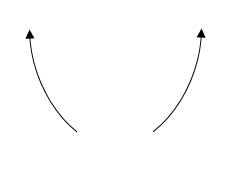
\includegraphics[width=0.3\textwidth]{../Figures/polyEndBehaviorCopyCC.png}
\end{center}\begin{enumerate}[label=\Alph*.]
\begin{multicols}{2}
\item 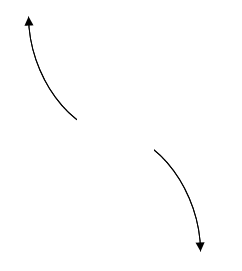
\includegraphics[width = 0.3\textwidth]{../Figures/polyEndBehaviorCopyAC.png}
\item 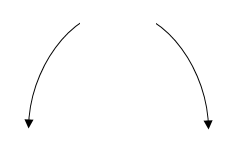
\includegraphics[width = 0.3\textwidth]{../Figures/polyEndBehaviorCopyBC.png}
\item 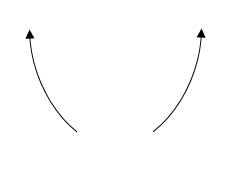
\includegraphics[width = 0.3\textwidth]{../Figures/polyEndBehaviorCopyCC.png}
\item 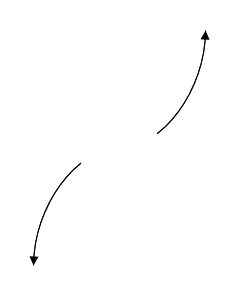
\includegraphics[width = 0.3\textwidth]{../Figures/polyEndBehaviorCopyDC.png}
\end{multicols}\item None of the above.\end{enumerate}
\textbf{General Comment:} Remember that end behavior is determined by the leading coefficient AND whether the \textbf{sum} of the multiplicities is positive or negative.
}
\litem{
Describe the zero behavior of the zero $x = -2$ of the polynomial below.
\[ f(x) = -8(x - 6)^{11}(x + 6)^{9}(x - 2)^{5}(x + 2)^{4} \]The solution is the graph below, which is option B.
\begin{center}
    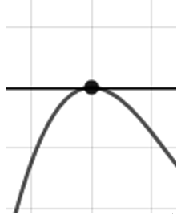
\includegraphics[width=0.3\textwidth]{../Figures/polyZeroBehaviorBC.png}
\end{center}\begin{enumerate}[label=\Alph*.]
\begin{multicols}{2}
\item 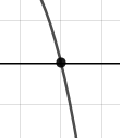
\includegraphics[width = 0.3\textwidth]{../Figures/polyZeroBehaviorAC.png}
\item 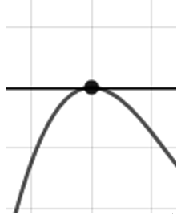
\includegraphics[width = 0.3\textwidth]{../Figures/polyZeroBehaviorBC.png}
\item 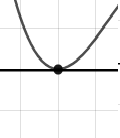
\includegraphics[width = 0.3\textwidth]{../Figures/polyZeroBehaviorCC.png}
\item 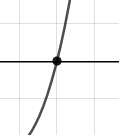
\includegraphics[width = 0.3\textwidth]{../Figures/polyZeroBehaviorDC.png}
\end{multicols}\item None of the above.\end{enumerate}
\textbf{General Comment:} You will need to sketch the entire graph, then zoom in on the zero the question asks about.
}
\litem{
Describe the zero behavior of the zero $x = -2$ of the polynomial below.
\[ f(x) = -4(x + 5)^{9}(x - 5)^{5}(x + 2)^{10}(x - 2)^{9} \]The solution is the graph below, which is option B.
\begin{center}
    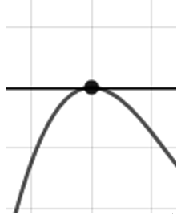
\includegraphics[width=0.3\textwidth]{../Figures/polyZeroBehaviorCopyBC.png}
\end{center}\begin{enumerate}[label=\Alph*.]
\begin{multicols}{2}
\item 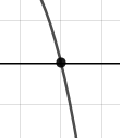
\includegraphics[width = 0.3\textwidth]{../Figures/polyZeroBehaviorCopyAC.png}
\item 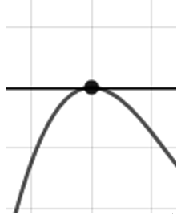
\includegraphics[width = 0.3\textwidth]{../Figures/polyZeroBehaviorCopyBC.png}
\item 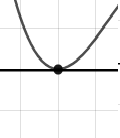
\includegraphics[width = 0.3\textwidth]{../Figures/polyZeroBehaviorCopyCC.png}
\item 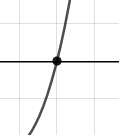
\includegraphics[width = 0.3\textwidth]{../Figures/polyZeroBehaviorCopyDC.png}
\end{multicols}\item None of the above.\end{enumerate}
\textbf{General Comment:} You will need to sketch the entire graph, then zoom in on the zero the question asks about.
}
\litem{
Which of the following equations \textit{could} be of the graph presented below?

\begin{center}
    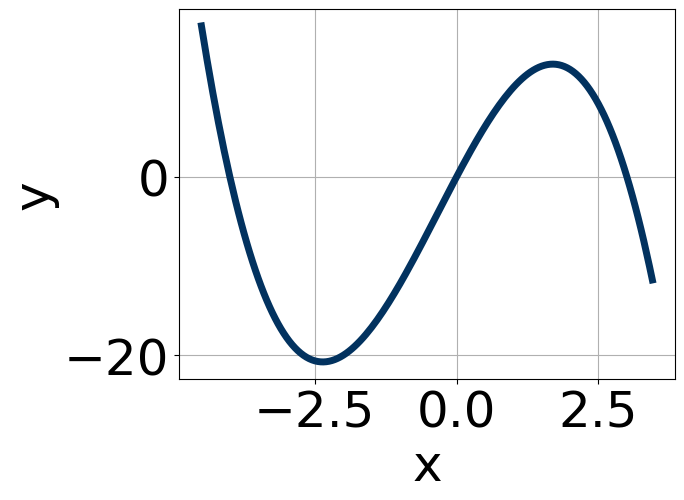
\includegraphics[width=0.5\textwidth]{../Figures/polyGraphToFunctionCopyC.png}
\end{center}


The solution is \( 19x^{6} (x + 3)^{8} (x + 4)^{11} \), which is option E.\begin{enumerate}[label=\Alph*.]
\item \( -18x^{10} (x + 3)^{6} (x + 4)^{8} \)

The factor $(x + 4)$ should have an odd power and the leading coefficient should be the opposite sign.
\item \( 7x^{5} (x + 3)^{6} (x + 4)^{6} \)

The factor $x$ should have an even power and the factor $(x + 4)$ should have an odd power.
\item \( -14x^{8} (x + 3)^{10} (x + 4)^{9} \)

This corresponds to the leading coefficient being the opposite value than it should be.
\item \( 2x^{5} (x + 3)^{10} (x + 4)^{7} \)

The factor $x$ should have an even power.
\item \( 19x^{6} (x + 3)^{8} (x + 4)^{11} \)

* This is the correct option.
\end{enumerate}

\textbf{General Comment:} General Comments: Draw the x-axis to determine which zeros are touching (and so have even multiplicity) or cross (and have odd multiplicity).
}
\end{enumerate}

\end{document}